\chapter[Technical and methodological background]{Technical and methodological background}
\label{background}
  \begin{verse}
    \textit{All the revision in the world will not save a bad first draft: for the architecture of the thing comes, or fails to come, in the first conception, and revision only affects the detail and ornament, alas!}\\
    \flushright{\textit{(T. E. Lawrence (1931))}}
  \end{verse}

The following two chapters will contain details about the planned system because an idea about the system, its behavior and the background of the used technologies is very important (just like the quotation above shows). 

In general, the planned application should be able to handle the complete workflow for a university course situation. So, the backend should offer features that offer groups of students the work on specific topics. The domain model showing this situation for a general university course is shown in Figure \ref{domain}. As one can see, students are working together in groups to create content for a specific topic. The whole process is supervised by the supervising employee of the university. 

\begin{figure}[th]
\centerline{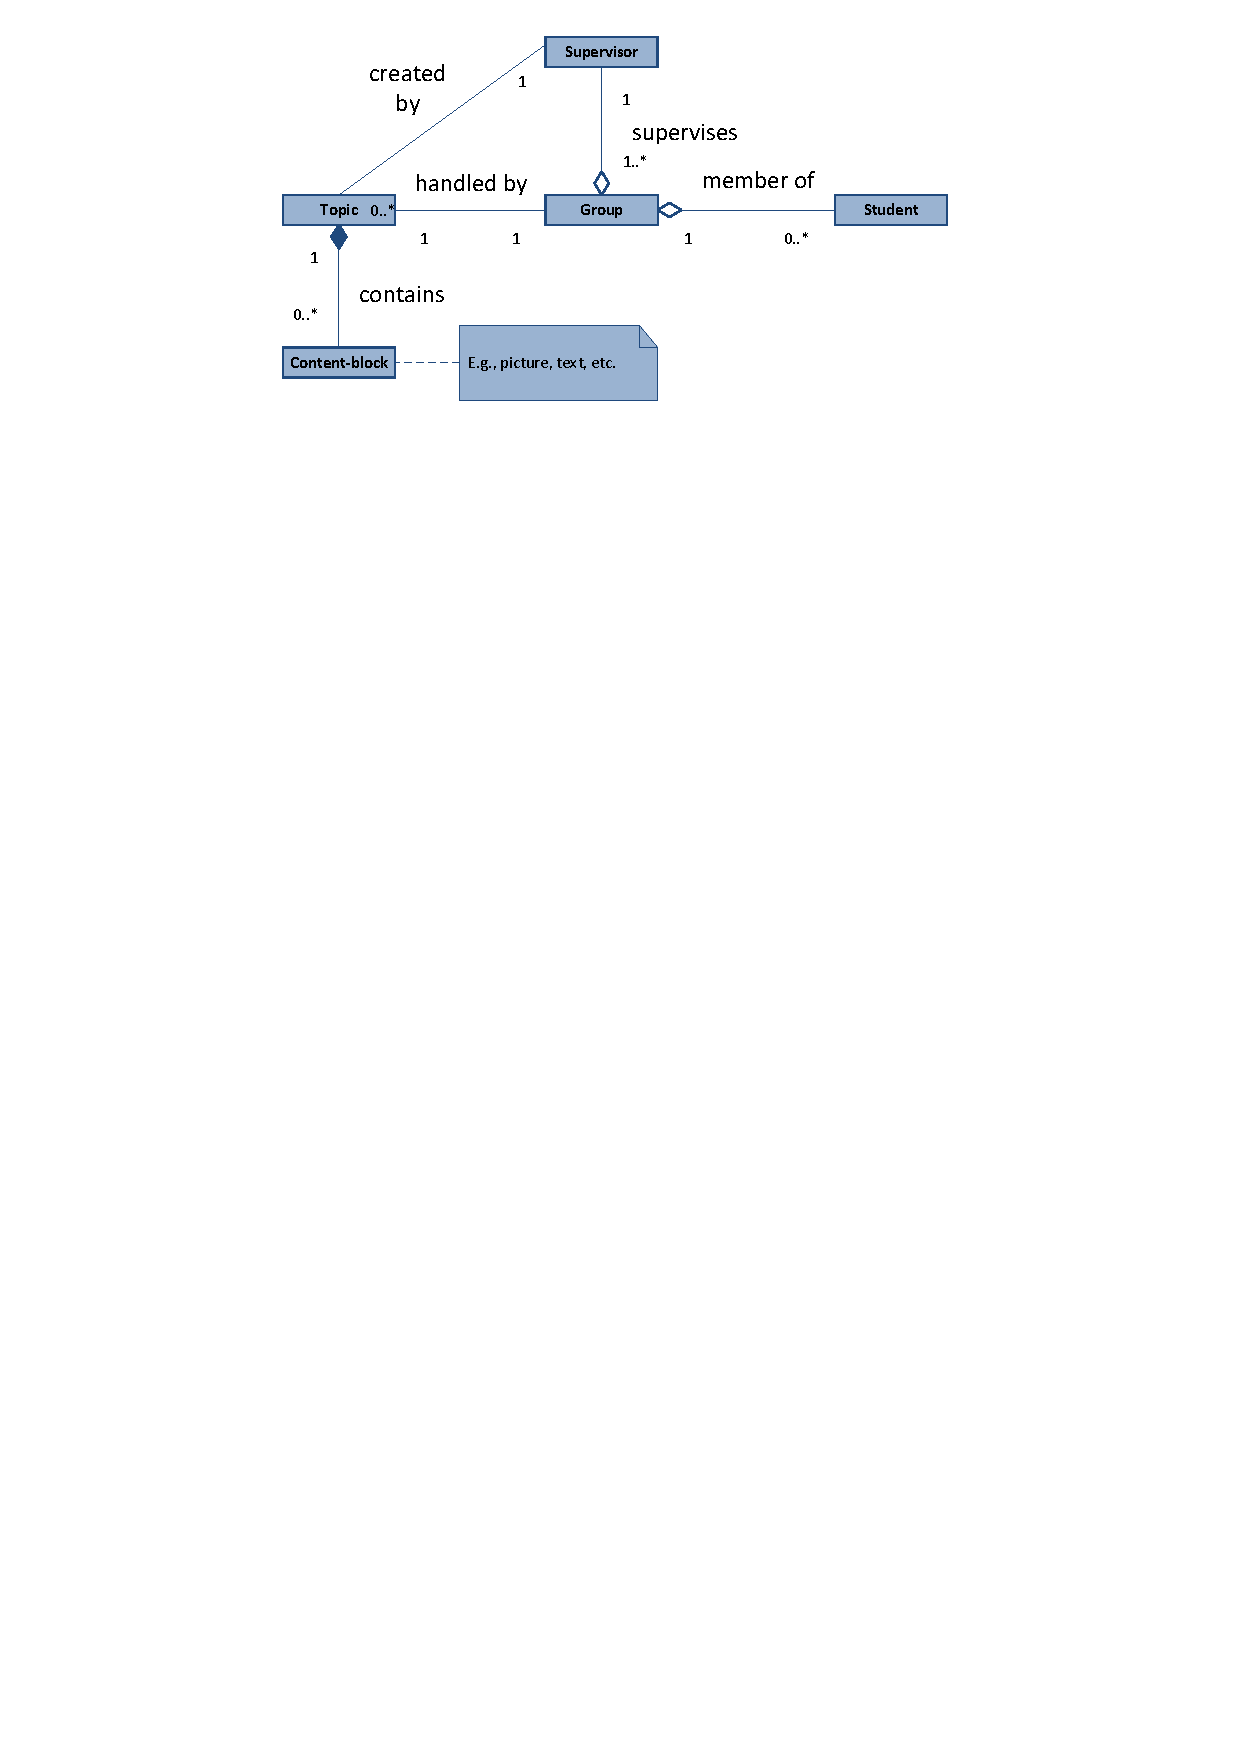
\includegraphics[width=1\textwidth]{gfx/domainModel.pdf}}
\caption{The domain model of the university courses.}
\label{domain}
\end{figure}

Before we come into more detail about the software itself, we will now get an insight into the used technical frameworks respectively tools and methodological concepts, which have been used during the development process.  Note that we will focus on the frameworks and plugins that are needed to understand the details of the implementation in chapter \ref{implementation}. Although, the whole system uses a lot more of them.

The first thing, which is important to notice, is that the system will be developed with an agile software development method, which will be based on Scrum. Because of that, we will start by explaining the Scrum development method.

\section{Agile Development - Scrum}
\label{SCRUM-intro}
The main idea of agile development is described within the agile manifesto \cite{Beck2001agile}\footnote{The whole manifesto can be found here: \url{http://agilemanifesto.org}}. Within agile development, the focus is set to frequent software delivery and close customer relationship. Because Scrum is such an agile development method, we find similar ideas in the Scrum development process. The HiP-application will be developed in a Scrum-like fashion to achieve a high efficiency in the small timeframe. However, a full Scrum approach is not possible because the development team is very small (i.e.,  we will combine different roles in one person). Nonetheless, we will include the ideas and concepts of the Scrum process. But to get a first intuition about the Scrum process itself, we will now describe the main ideas of Scrum and agile development in general.

Using Scrum means, the application will be developed within autonomous short \textit{sprints} with a length between 1 up to 4 weeks. However, \cite{Ber07} points out that a four week sprint is in many cases problematic because a lot of customer requests have to be included into currently running sprints and so the backlog becomes more and more useless; he suggests sprints with a length of about 2 weeks. In any case, after every sprint the product should be more refined (\cite{scrum}). Of course, it should be possible to execute the application at the end of any given sprint, which will result in a fast and stable development process. The general development process is also shown in Figure \ref{ScrumDia}. The Product-Backlog is the foundation of every sprint-backlog because it contains every feature that will be needed in the product at some time. So, one derives the sprint-backlog, which includes every feature that should be added in a specific sprint, from the product-backlog for every new sprint. In addition to that, daily Scrum meetings should ensure that the whole team is up-to-date and as efficient as possible. In more detail, Scrum is known to reduce every category of work (i.e., defects, rework, total work required, and process overhead) within a \ac{CMMI} compliant development process by almost 50\% (\cite{Sut09}), which is also great for development in the short timeframe of the master thesis. The close customer relationship can for example be found in the fact the the customer is often invited in meetings after the sprints to see the progress on the product and, more important, to be able to influence the development process. However, \cite{paulk2002agile} claims that customers may also create a threat to finish agile development successful if they are not able or willing to maintain such a close relationship with the development team.

We will use a \ac{TDD}-like approach within every sprint (where possible) because we will need to adapt and refactor existing code often. So, we will at first create needed test cases and afterwards implement against these test cases. This approach will prevent that testing of the application will be shifted into the last week(s) of the development process and done in a superficial way. In addition to that, a comprehensive test suite is a great basis for further development (\cite{max03}).

\begin{figure}[th]
\centerline{\includegraphics[width=1\textwidth]{gfx/scrum}}
\caption{The Scrum development process (Simplified, original work from \cite{5_maxxor.com_2015}).}
\label{ScrumDia}
\end{figure}

Now, after we have seen the general concept of Scrum, we will now take a look at methods for cost estimation. 

\section{Methods for cost estimation}
\label{cost}
To get a feasible estimation of the workload of a given backlog, as it has been described in section \ref{SCRUM-intro}, we need some methods to create a good work- respectively cost-estimation. This is important to be able to choose a fitting amount of work per sprint.

As \cite{Keaveney11} points out, one of the main principles of agile methods is to have meetings with the customer within the development phase to adapt the requirements if needed (\cite{beck2001agile}). However, changing requirements within a currently running software development are a common cause of problems with respect to software cost estimating (\cite{jones2003flawed}). So, our methods for cost-estimation has to be able to handle changing requirements in short time-frames. Similarly, surveys have shown that in real life scenarios, the techniques used to estimate costs in agile development projects are in general based on the expertise of the team-members (\cite{ceschi2005project}). So, the developers look to past iterations (or even past projects) to produce estimates about the costs of the current project respectively sprint (\cite{ceschi2005project}). 

To be able to formalize knowledge about past iterations and to be able to compare the data with the current iteration, one can use diagrams like burn-down charts.

\subsection{Burn-down charts}
To get the idea of burn-down charts, we need a first intuition about story points. Story points correspond to a specific estimated time-frame, like one story point per 30 minutes \emph{- Story points will be explained in the next section. For now, see them as a unit of needed time - }.

A burn-down chart shows the amount of remaining story points on the y-axis and the days of the sprint on the x-axis. With such a chart, one can estimate the remaining time and can derive if the sprint can be finished in the given time-frame by looking at the \textit{slope} of the graph. Figure \ref{Burndown example} shows an example burn down chart over 8 days. The OPT line shows the optimal slope that ends up on 0 remaining story points on the last day. If the sprint curve is above the OPT line, the developers are to slow in the current sprint and in the case the sprint curve is below the OPT line, the developers are ahead of the time. 

Obviously, burn-down charts do not have problems with changing requirements outside of the current sprint. 
But, in addition to that, we can also include new tasks to a running sprint and can simply adapt the OPT line with its slope to track the new added tasks within the active sprint. With this knowledge about the management of tasks and time estimation, we can take a closer look at story points.

\begin{figure}[th]
\centerline{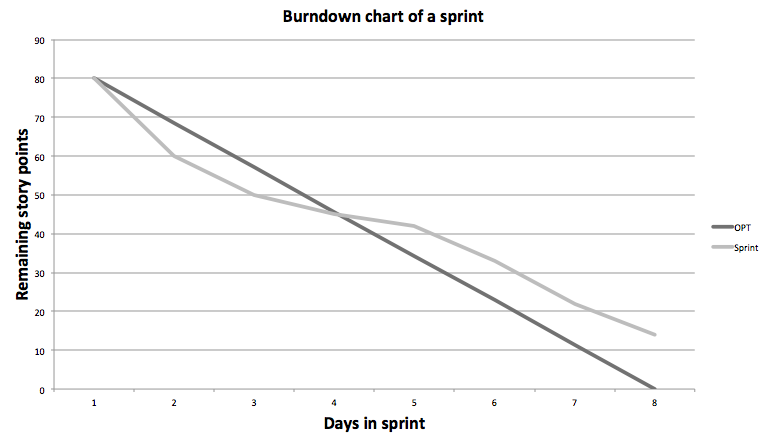
\includegraphics[width=1\textwidth]{gfx/burndown}}
\caption{A burn-down diagram showing an example sprint.}
\label{Burndown example}
\end{figure}

\subsection{Story points}
\label{storyPoints}
In the previous section we have implicitly used the unit  \emph{story points}. Story points are tightly coupled with the idea of agile development because they represent an unit of needed time that takes the team members effort and the subjective degree of difficulty into account (\cite{ScrumMeth}). This cannot be done by a manager, who is estimating the time and assigning tasks based on conjectures about the performance of the team. The main idea about story points is that the actual amount of time, which is expressed by a story point, does not matter. The important thing is that the collaborating teams share a common understanding of its scale. So, every team-member should be comfortable with the represented time. 

Another idea is that you can easily imagine the analogy 'this story is like that story, so it well take about the same time', which tries to improve the quality of time estimations (\cite{cohn2004user}).

Now, as we have seen how to manage the reduction of requirements with burn-down charts and story points, we will take a look at the way we can specify user requirements in the first place; by using user stories.

\subsection{User stories}
As \cite{Pichler:2010aa} describes, a user story explains how a customer or a user uses the final the product in a short story. To create respectively discover these stories, one can use personas. Such a persona is a fictional character that represents a specific user type that might use a website or a product. A persona for our \ac{HiP} backend could for example be \emph{Steve}, the 24 year old student of english history that needs to create his homework with the backend. Obviously, Steve would represent the role \emph{student} from the view of the backend. 

Another important fact about user stories is that they are closely related to agile development. This relation can, for example, be seen at the fact that each user story is expected to result in a contribution to the value of the general product. This contribution should be added regardless of the order of the actual implementation (\cite{Alliance:2013aa}). Of course, this is a necessary condition for a user story, if one thinks about the way the development team works on the backlog of the product. The entries within the backlog are sorted into sprints and each entry within a sprint can be implemented as an autonomous unit by the development team. So, in general, one do not have any dependencies on entries within the sprint backlog.

\section{DevOps}
Besides the cost estimation and requirement engineering, the deployment process is an important detail within the software development process. It determines the speed in which new features are shipped to the customer (respectively released to an online service, which is in general the same).

Now, the term \emph{DevOps} can be seen as the practice of \emph{operations} and \emph{development} (-engineers) participating together in the entire service lifecycle, from design through the development process to production support (\cite{Mueller2011}). This approach is, for example, used by Netflix, Amazon and Etsy to deliver their new features in a fast way to the enduser (\cite{duvall2012breaking}).

Using a DevOps approach results in a couple of benefits like the fact that one learns about the induced problems much faster because one gets much faster feedback from the enduser. Obviously, it is easier to fix a bug in such a situation, as in the case that the customer detects a bug in a 'new' release, which is four month old on the development machines. This results also in the benefit that the problems are much smaller and need less time to be fixed (\cite{duvall2012breaking}).
Furthermore, the focus on DevOps leads to the usage of tools that offer the possibility for new ways of structuring the architecture of the system (\cite{cukier2013devops}). One of these approaches is the fact that, as soon as one starts thinking in much smaller autonomous chunks, it becomes much easier to migrate the developed system into a cloud service in a \ac{PaaS} like fashion (\cite{cukier2013devops}). 

One of the tools you need to create a DevOps process (respectively a DevOps culture), is \acl{CD}.

\subsection{Continuous Delivery and Continuous deployment}
\acf{CD} is the automated implementation of the build, deploy, test and release process. A \ac{CD} process runs the software tests on every version that is committed to the version-control system and provides a quick automated feedback on the test result. By using a \ac{CD} process, the release of a new software version becomes easy and fast. 

Thus, \ac{CD} is the needed brick for creating a \emph{continuous deployment process}. Within such a process every commit that is done by the developer and send to the code-versioning software becomes automatically shipped to the enduser (or at least parts of them - like only in North America for a specified time) by the \ac{CD} system. However, a continuous deployment process cannot be used in every situation but can be a very important thing for fast paced companies like Netflix or Flickr. The complete process is also shown in Figure \ref{hip:cd}. As one can see within this figure, the process is quite straight forward and can easily be automated by using tools and platforms like \emph{Bamboo} and \emph{GitHub}.

\begin{figure}[th]
\centerline{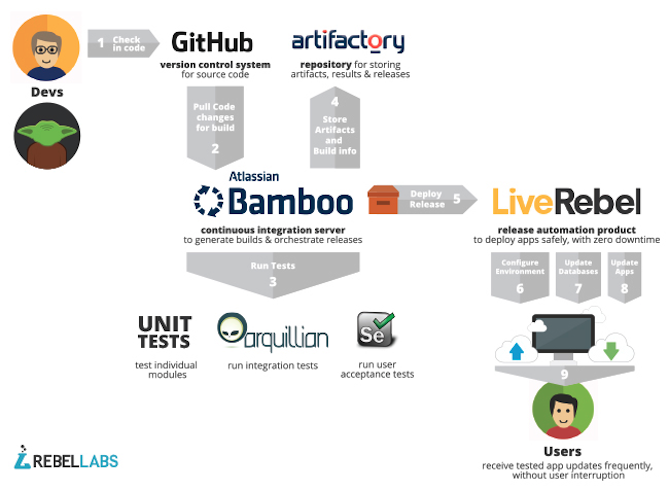
\includegraphics[width=1\textwidth]{gfx/continuous-delivery}}
\caption{The \ac{CD} process showing some tools that can be used to create a \ac{CD} pipeline (taken from \cite{Wattson:2013aa})}
\label{hip:cd}
\end{figure}

Now, after we have gained some insights about the process itself, we will take a look at the frameworks that will be used in the development process.

\section{Used Frameworks}
Because the time frame for the project is quite small, it is not possible to create the whole application from scratch and, thus, we need a couple of frameworks to accelerate the process. We will use the Play-Framework in the backend, which offers a \ac{HTTP}-interface and handles the routing from \ac{HTTP}-requests to application code. On the frontend-side, AngularJS will be used to create a fast and responsive web-interface and Junaio will be used to include the \ac{AR}-functionality on the smartphone application.

\subsection{Play Framework}	
\label{Play2}
We will use the Play framework for the backend of the application because Play is an open source web application framework, which is written in Scala and Java, follows the \ac{MVC} architectural pattern and handles the routing from \ac{HTTP}-requests to application code. 

A simple example for the routing configuration file is shown in Listing \ref{Play:Routing}. In this file, each documented route consists of an \ac{HTTP} method and an \ac{URI} pattern that is linked to a call of a, so called, \textit{action method} within the Java respectively Scala code. 

As one can easily see in line 9, it is quite easy to pass parameters to the application code. Furthermore, one can see that the parameters are type-safe. Thus, for example, a String passed in as an Integer would result in a compilation error. 

\lstset{language=XML,
basicstyle=\small,
showspaces=false,
showstringspaces=false,   
tabsize=2,
backgroundcolor=\color{grey}}
\begin{lstlisting}[numbers=left,caption={Simple routing configuration file within the Play Framework},label=Play:Routing,frame=tlbr,breaklines]
# Routes
# This file defines all application routes (Higher priority routes first)
# ~~~~

# Home page
GET /               controllers.Application.index()

# Usage of parameter
GET /thesis/:grade  controllers.Application.exp(grade: Integer)

# Map static resources from /public to the /assets URL path
GET /assets/*file   controllers.Assets.at(path="/public", file)
\end{lstlisting}

Very briefly, the Play framework includes three different parts: 

1) Java code that implements the controllers. The controllers are used to handle requests that get routed to them via \ac{HTTP}. A simple controller is shown in Listing \ref{Play:Controller}. As one can see within line 10 of Listing \ref{Play:Controller} the String "Your new application is ready" gets passed to the render function of the class index and returned as a parameter within the \textit{ok} function, which creates a simple \ac{HTTP} header with return-code 200. The index class is a Scala class that gets automatically created from the Scala/\acs{HTML} template called \textit{index.scala.html}. We will see this in more detail within point 3 of this list.

\lstset{language=Java,
basicstyle=\small,
showspaces=false,
showstringspaces=false,   
tabsize=2,
backgroundcolor=\color{grey}}
\begin{lstlisting}[numbers=left,caption={Simple Java-controller within the Play Framework},label=Play:Controller,frame=tlbr,breaklines]
package controllers;

import play.*;
import play.mvc.*;
import views.html.*;

public class Application extends Controller {

    public static Result index() {
        return ok(index.render("Your new application is ready."));
    }
}
\end{lstlisting}

2) Java code that implements the model entities. The model in Play 2.0 is used to do the data handling, which is quite easy because the Play framework maps automatically the documents in the MongoDB to concrete Scala ojects. \\
3) Scala templates that are used as \textit{views}. As a return value of the controllers, they pass data to a fitting template and return a corresponding \ac{HTML}-view. However, we may also skip the template engine sometimes to directly return \ac{JSON}-documents, which can be used to provide a \ac{API}. Listing \ref{Play:Template} shows the used \textit{index.scala.html} template used in Listing \ref{Play:Controller}. In line 1 of Listing \ref{Play:Template}, we declare the used parameters (i.e., a String variable) that we have used to pass the String "Your new application is ready". The \textit{@main} command in line 3 calls another template, which includes everything besides the \ac{HTML} body. The body of the file is now included in line 4 by calling another framework specific method, which includes a welcome and documentation message and renders our passed String variable.

\lstset{language=XML,
basicstyle=\small,
showspaces=false,
showstringspaces=false,   
tabsize=2,
backgroundcolor=\color{grey}}
\begin{lstlisting}[numbers=left,caption={Simple Scala template within the Play Framework},label=Play:Template,frame=tlbr,breaklines]
@(message: String)

@main("Welcome to Play") {
    @play20.welcome(message, style = "Java")
}
\end{lstlisting}

Besides the templating feature, Play can be augmented with Plugins that handle specific behavior. For example, the Plugin \emph{SecureSocial 2} is able to handle the whole user registration and login process. In more detail, it offers an interface to get the data from users, who are currently logged into the system. Furthermore, it offers out of the box support for web-services like Twitter, Facebook, Google, LinkedIn and GitHub. If one do not want to rely on external services, \emph{SecureSocial 2} provides a Username/Password mechanism with signup, login and reset password functionality. We will use this last technique within the \ac{HiP} backend.

As another important fact, Play emphasizes the usage of the \ac{REST} principle, as it can be seen within the routing configuration file. We can easily and directly make use of the different \ac{HTTP} commands and use them to structure our \ac{API} accordingly. In general, \acf{REST} is a style of software architecture that is used to build distributed systems and has been introduced in the dissertation of \cite{Fielding2000}.

The core ideas of \ac{REST} are:  
\begin{itemize}
\item A resource is identified by a persistent identifier (i.e., the \ac{URI}).
\item A resource (on the server side) is manipulated by using the fitting \ac{HTTP} methods: POST, GET, PUT, and DELETE. So, one should not use \ac{HTTP} GET to change something on the server.
\item The actual representation, which gets downloaded as a resource from the server, is dependent on the request itself and not the used identifier. As stated in the first point of the list, every identifier identifies exactly one concrete resource. So, one should use \ac{HTTP} Accept headers to control the needed representation (e..g, \ac{XML}, \ac{JSON}, etc.).
\end{itemize}

As Rodriguez et. al. point out, \ac{REST} based web services are easier to use than \acf{SOAP} and \acf{WSDL}-based ones and getting more and more importance since mainstream web 2.0 service providers (i.e., Facebook, Twitter, etc.) are taking up on \ac{REST} (\cite{Rodriguez2008}). Besides the \ac{REST} support, the Play-framework comes with integrated unit testing and full support of asynchronous I/O.  So, all in all, Play will noticeably enhance the development speed of the backend.

\subsection{MongoDB}
MongoDB is a document-oriented database, which stores data as \ac{JSON} objects. Thus, data entries within the MongoDB are called documents and are in essence ordered sets of key-value pairs (\cite{Tre14}). However, values can also be complete documents and arrays. So, one can store complex hierarchical structures within a MongoDB. Similarly, binary data (e.g., pictures) gets stored in a \ac{BSON}-format. This format is a binary \ac{JSON} format that includes datatypes and better traversability.

These documents are stored in \emph{collections}, which are in general comparable to the tables in a relational database, like MySQL.

Every document within the database needs to include a field called \textit{\_id}, which contains the primary key of the document. Of course, this primary key has to be unique within the collection that contains the document. If an document is stored within the database without an \textit{\_id} field, the field gets automatically generated.

An insert into a MongoDB is easily done and shown in Listing \ref{MongoDB:insert}. 

\lstset{language=JavaScript,
basicstyle=\small,
showspaces=false,
showstringspaces=false,   
tabsize=2,
backgroundcolor=\color{grey}}
\begin{lstlisting}[numbers=left,caption={Inserting into a MongoDB},label=MongoDB:insert,frame=tlbr,breaklines]
var db = ... // contains the connection to the database

var object = {
	firstname : 'John',
	lastname : 'Doe'
};

db.hipUsers.insert(object);
\end{lstlisting}

Similarly one can read documents from the database by creating a document that is matched against the collection.
For example, to retrieve the user \textit{John Doe} that has been included within Listing \ref{MongoDB:insert} by matching against his lastname, one would need to do the steps shown in Listing \ref{MongoDB:query}. The object that is used to match the query is created in line 3. The query itself is started in line 7 of Listing \ref{MongoDB:query}.

\begin{lstlisting}[numbers=left,caption={Reading documents from a MongoDB},label=MongoDB:query,frame=tlbr,breaklines]
var db = ... // contains the connection to the database

var object = {
	lastname : 'Doe'
};

db.hipUsers.find(object);
\end{lstlisting}

Within the following section, we will take a look at the frontend technologies.

\subsection{AngularJS}
\label{AngularJS}
After we have now seen the basics of the Play framework and the MongoDB, which will handle the backend functionality, we will now take a look at \textit{AngularJS}, which will provide needed features to create a fast and responsive frontend. The frontend will be designed as a \ac{SPA}. A \ac{SPA} is an orthogonal approach to the common way of creating websites as a set of linked pages. A \ac{SPA} is a composition of individual components which can be updated respectively replaced independently of the complete site and, thus, without any reload after the actions of the user. This results in a couple of benefits, like improved interactivity, responsiveness and user satisfaction (\cite{Mes07}). Another important fact with respect to the system performance is that AngularJS offers functions (as we will see: \emph{directives}) to circumvent the need for changing the \ac{DOM}-Tree directly. AngularJS relies on a \ac{MVVM} architecture and tries to create the same behavior by doing changes to the ViewModel. The ViewModel sits behind the concrete \ac{UI} layer and exposes data needed by a View from a Model. Because of that, the ViewModel can be viewed as the source of data for the Views to get data and call functions. 

\lstset{language=JavaScript,
basicstyle=\small,
showspaces=false,
showstringspaces=false,   
tabsize=2,
backgroundcolor=\color{grey}}
\begin{lstlisting}[numbers=left,caption={Simple example that shows the use of an AJAX request that shows the response text within a specific div container},label=AJAX:Example,frame=tlbr,breaklines]
xmlhttp.onreadystatechange=function(){
  if (xmlhttp.readyState==4 && xmlhttp.status==200){
    document.getElementById("myDiv").innerHTML=xmlhttp.responseText;
    }
  }
xmlhttp.open("GET","ajax_info.txt",true);
xmlhttp.send();
\end{lstlisting}

Obviously, creating a \ac{SPA} implicitly forces the usage of some kind of request mechanism to get the data that the user needs without reloading the site. This could for example be done with an \ac{AJAX} request like the one that is show in Listing \ref{AJAX:Example}. The listing shows how the request is being made in line 6 and 7. Line 3 shows the exchange of the content of the div container with the id \textit{myDiv}. However, using \ac{AJAX} is cumbersome and can nowadays easily be hidden in very sophisticated frameworks, like AngularJS.

The \textit{AngularJS} framework will be explained briefly in the following. AngularJS makes heavy use of expressions and directives.
While directives in AngularJS are functions that get run when the DOM is compiled by the compiler and are shown as simple tags or attributes, an expression is a term that is encapsulated by \textit{\{ \{ ... \} \}} and gets evaluated while the page gets loaded. Listing \ref{Angular:expressions} shows a simple example, where an expression is used to call a method of a controller object.

\lstset{language=XML,
basicstyle=\small,
showspaces=false,
showstringspaces=false,   
tabsize=2,
backgroundcolor=\color{grey}}
\begin{lstlisting}[numbers=left,caption={Simple example that shows the use of expressions},label=Angular:expressions,frame=tlbr,breaklines]
<div class="panel-heading"> 
	{{lc.getTerm('system_group_navigation')}} 
</div>
\end{lstlisting}

As soon as the page gets rendered, the \ac{DOM}-tree will be loaded with the result value of the given javascript function called \textit{getTerm(String)}. 
Another major feature of AngularJS is the, so called, two-way data binding. This feature is closely coupled to expressions. The two-way data binding ensures that the rendered value of the function getTerm(String) gets automatically updated, as soon as the function returns a different value. This creates a source-code that includes less unnecessary lines of code for updating the values in the view. 

Furthermore, AngularJS offers directives like \textit{ng-class} which adds dynamically a specific class to a \ac{DOM}-element if a given expression evaluates to true.

\lstset{language=XML,
basicstyle=\small,
showspaces=false,
showstringspaces=false,   
tabsize=2,
backgroundcolor=\color{grey}}
\begin{lstlisting}[numbers=left,caption={Simple example that shows the ng-class directive to change the style respectivly color of an alert depending on its type},label=Angular:ngclass,frame=tlbr,breaklines]
<div ng-class="{'alert-warning' : alert.type == 'warning',
                         'alert-danger' : alert.type == 'danger',
                         'alert-info' : alert.type == 'info',
                         'alert-success' : alert.type == 'success'}"
     role="alert">

	{{alert.msg}}
</div>
\end{lstlisting}
Listing \ref{Angular:ngclass} shows how the \textit{ng-class} directive exchanges the used style of the alert depending on the boolean expression that is places behind the ':'. So, the syntax of the attribute value is \{ class : expression \}.

Of course, one can also create own directives to get a much cleaner code. For example, it is possible to create a directive called \textit{chat-box} that can directly be included within the \ac{DOM}-tree. Thus, the usage of the created chat element folds down to the code that is shown in Listing \ref{Angular:ownDirective}. The same can be achieved by using web components or Google Polymer, which is in essence an extension of the web-components technology. However both technologies are, at the present point in time, only fully compatible to Google Chrome. Because of that, we will use custom AngularJS directives to create clean and maintainable code.

\lstset{language=XML,
basicstyle=\small,
showspaces=false,
showstringspaces=false,   
tabsize=2,
backgroundcolor=\color{grey}}
\begin{lstlisting}[numbers=left,caption={Simple example that shows the usage of a custom directive},label=Angular:ownDirective,frame=tlbr,breaklines]
<!-- some code up here -->

<chat-box> </chat-box>

<!-- some code down here -->
\end{lstlisting}

Besides AngularJS, Twitter Bootstrap will also play an major role in the frontend development process.
 
\subsection{Twitter Bootstrap}
Twitter Bootstrap\footnote{Twitter Bootstrap is hosted on GitHub and can be downloaded here: \url{https://github.com/twitter/bootstrap}} is an open and freely available collection of tools on the basis of the \ac{HTML}, \ac{CSS} and \ac{JS} and can be used to support and accelerate the creation of web applications. We will use Twitter Bootstrap inside the user front-end of our web application because it works nicely together with AngularJS and can for example be used to create tabs and alerts. Furthermore, Twitter Bootstrap is nowadays used by a lot of common web-applications. Thus, we enhance the external consistency of the \ac{HiP}-application in respect of other web-applications (\cite{lidwell2010universal}), which may be well known to the user. 

Twitter Bootstrap is licensed under the terms of the Apache License v2.0\footnote{The terms of the license can be found here: \url{http://www.apache.org/licenses/LICENSE-2.0}}.

Furthermore, Twitter Bootstrap can be used with Bootstrap UI, which are Bootstrap components that have been written in AngularJS and can easily be reused. Examples for these components are tooltips, datepickers, timepickers, etc. So, this is also a great repository for components to accelerate the development process. \footnote{Bootstrap UI can be downloaded here: http://angular-ui.github.io/bootstrap/ and is distributed under the MIT license https://github.com/angular-ui/bootstrap/blob/master/LICENSE}

\subsection{Junaio - Metaio}
\label{AREL}
The \ac{AR}-functionality will be offered by the framework Junaio. The company Metaio, which runs Junaio, offers a developer program to develop own applications on the basis of the Junaio (eco-)system. Moreover, it is completely free of charge for the developers (\cite{junaio1}). However, deployed apps will be shipped with a Metaio watermark inside as long as you do not buy a specific license. 

\begin{figure}[th]
\centerline{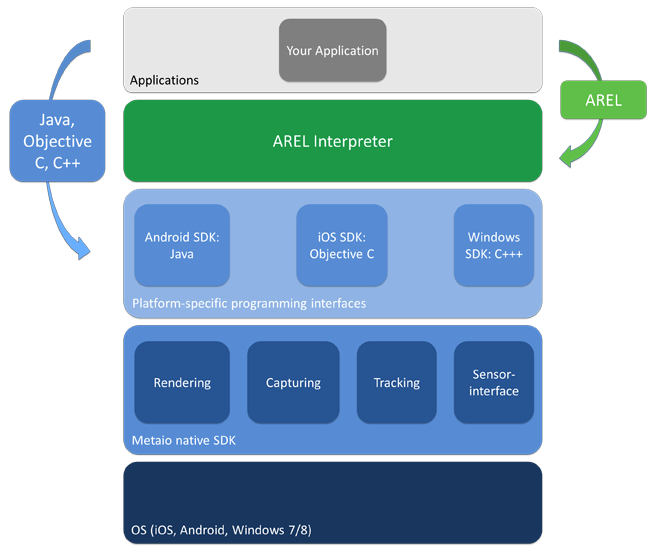
\includegraphics[width=.7\textwidth]{gfx/stackAREL}}
\caption{The figure shows the placement of the AREL interpreter within the platform stack. (Taken from \cite{MetaioDEV})}
\label{stackArel}
\end{figure}

Furthermore, Metaio has developed a JavaScript binding of the SDK used for \ac{AR}-applications called \ac{AREL}, which can be used as a platform to write your \ac{AR} apps without writing platform specific code of the mobile operating system \cite{MetaioDEV}. Figure \ref{stackArel} shows the placement of the \ac{AREL} interpreter within the platform stack. 

To use \ac{AREL}, we need three different parts that that get combined to an \ac{AREL} application.

\lstset{language=XML,
basicstyle=\small,
showspaces=false,
showstringspaces=false,   
tabsize=2,
backgroundcolor=\color{grey}}
\begin{lstlisting}[numbers=left,caption={Example for the HTML5 AREL layer},label=AREL:HTML5,frame=tlbr,breaklines]
<head>
   <!-- Integrates the arel javascript bridge -->
   <script type="text/javascript" src="http://dev.junaio.com/arel/js/arel.js"></script>

   <!-- Includes application logic -->
   <script  type="text/javascript" src="logic.js"></script>
</head>
\end{lstlisting}

First of all, we need a static content definition, which is an \ac{XML} document that references the models and graphics that will be loaded when we start the \ac{AREL} application. The second part is the \ac{HTML5} layer, which is also addressed in the static content definition. The \ac{HTML5} binds the static content definition to the application logic and may also add additional \ac{GUI} functionality. An example for such an \ac{HTML5} layer is shown in \ref{AREL:HTML5}. The last part, the application logic is written in \ac{JS} and loads objects that are afterwords tracked by patterns.  

So, \ac{AREL} allows scripting of \ac{AR}-applications on mobile operating systems like iOS or Android based on common web technologies such as \ac{HTML5}, \ac{XML} and JavaScript. 

\subsection{WebGL and JSModeler}
Last but not least, we will need \ac{WebGL} to create a possibility to render and manipulate the 3D-point clouds, of the scanned objects, right within the browser. However, we will use libraries like \emph{JSModeler} to abstract from the low-level OpenGL commands and simplify the development process.

JSModeler provides a 3d object viewer for presenting 3d models and small scenes on a web page. It is able to import models with the formats 3DS, OBJ and STL. Furthermore, it is able to manipulate the points within the internal buffer, so we will be able to manipulate rendered objects. 

After we have now taken a look at the used frameworks and technologies, we will now change our view to the used techniques and tools.

\section{Testing techniques and tools}	
Because we use an agile development approach, testing becomes an important aspect even in the development process itself. This founds on the core aspect of agile development that even in early stages of the development process the requirements are going to slightly change and, thus, we need to adapt the existing code. This leads us to \ac{TDD}, which is a developing technique that relies on the heavy use of tests. \ac{TDD} will be explained in the following section. 

\subsection{TDD}
The main idea of \ac{TDD} is that one develops the test cases upfront and implements the needed functions afterwards. This is a major shift in the way software gets developed as, traditionally, unit testing has been done on exiting code, after it has been implemented. According to \cite{nerur2005}, this \ac{TDD} approach leads to code that is more understandable and maintainable. However, \ac{TDD} is not only a different testing technique. As the definition of the Agile Alliance (\cite{GAA2015}) states \textit{"Test-driven development" refers to a style of programming in which three activities are tightly interwoven: coding, testing (in the form of writing unit tests) and design (in the form of refactoring)}. 

So, \ac{TDD} is not only a testing technique, it is a programming technique which follows a couple of rules to achieve a tight coupling of coding, testing and design. While the two parts coding and testing are easy to grasp, the relation between writing test cases and designing a system seems to be a bit odd. However, as \cite{Janzen2005} point out, while writing a test one is deciding what the program should do, which is an analysis step. This is how analysis gets coupled with testing.

Furthermore, \cite{Janzen2005} state that the positive aspects of the usage of \ac{TDD} has also been shown in studies of the \ac{NCSU}, which has performed a couple of empirical studies (\cite{George2004}, \cite{max03}, \cite{Williams2003}) on TDD in industry settings.
These studies showed that programmers, who used \ac{TDD} to produce code, created 18 up to 50 percent more external test cases than code that has been produced by corresponding control groups. The studies also reported that the \ac{TDD} developers spent less time while debugging their code. Nevertheless, they reported also that the \ac{TDD} project took up to 16 percent longer. But, in the case that took 16 percent more time, researchers noted that the control group without \ac{TDD} wrote far fewer tests than the \ac{TDD} group. 

According to \cite{GAA2015} the \ac{TDD} process can be expressed with the following set of steps:

\begin{enumerate}
  	\item write a \emph{single} unit test describing an aspect of the program
  	\item run the test, which should fail because the program lacks that feature
  	\item write \emph{just enough} code, the simplest possible, to make the test pass
	\item \emph{refactor} the code until it conforms to the \textit{simplicity criteria}
	\item repeat, \emph{accumulating} unit tests over time
\end{enumerate}

Note that the \textit{simplicity criteria} within step 4 of the procedure has been defined by \cite{Beck1999} as: \textit{At every moment, the design runs all the tests, communicates everything the programmers want to communicate, contains no duplicate code, and has the fewest possible classes and methods. This rule can be summarized as, ''Say everything once and only once.''}. 

So, all in all, the \ac{TDD} process relies on writing unit test before writing the application code itself and use them as tests in the developing phase to check if the currently written code is able to fulfill the requirement. Step 5 shows, that the sum of all test cases is then also used in a \textit{traditional} way to find bugs in the existing application-code. 

\subsection{Jasmine and Karma}
As we have seen in the last section, testing will be a major part of the development process. Thus, the chose of a good test environment is important. Karma is a test runner, which can be extended with a couple of plugins (e.g., code-coverage, more available browsers, etc.) that allows you to execute JavaScript code in multiple real browsers. The tool has been created by the team that has created AngularJS and is, thus, suggested as the main test runner within an AngularJS environment (\cite{7_github_2015}).  

Furthermore, Karma can be used with an extension called \emph{Karma-jasmine} to run Jasmine test cases. \emph{Jasmine} is a behavior-driven testing framework that can be used to test JavaScript code. As a brief explanation, \ac{BDD} is a development method that has been evolved from \ac{TDD} to get the idea to a bigger audience and to shorten the gap between behavior (which can easily be explained to the customer) and code (\cite{BDD}). Thus, we will use Karma with the Jasmine extension to run our Jasmine test case for the application.
 
\section{Tooling}
A couple of frameworks and techniques is a good start for creating such a sophisticated system. However, we will also need fitting tooling to support the development. These tools will be described in the following section.

\subsection{Git}
We will use Git, which is a commonly used distributed revision control and source code management system, for the versioning of our source-code. Git is free software distributed under the terms of the GNU General Public License version 2.

The service GitHub offers his users the possibility to maintain public and private Git repositories. The usage of GitHub is free, if the user uses public repositories only. We will use GitHub to host our source-code.

\subsection{Jira}
Jira is a proprietary software for project tracking purposes, which has been developed by the company Atlassian. It has support for agile development methods like Scrum or Kanban and offers a couple of features for bug tracking and time respectively cost estimation, like burn-down charts, which has been explained in section \ref{cost}. 

We will use Jira to track the status of the \ac{HiP} application.

\subsection{IntelliJ IDEA}
IntelliJ IDEA is a Java \ac{IDE} by the company JetBrains. 

The current version offers support for Java 8, UI designer for Android development, Play 2.0 and Scala and is, thus, a good choice to work with because all of these features will be used in our development process.

The \ac{IDE} is available as an Apache 2 Licensed community edition and a commercial edition. The commercial edition can also be downloaded for free for educational purposes.

After we have now seen all needed fundamentals to grasp the main idea of the application, we will take a look at the draft of the application.